\documentclass[12pt]{article}
\usepackage{fullpage}
\usepackage{csquotes}
\usepackage{underscore}
\usepackage{url}
\usepackage{graphicx}
\usepackage{caption}
\usepackage{array}
\usepackage{amsmath,amsfonts,amssymb}
\usepackage{multirow}
\usepackage{indentfirst}
\setlength{\parindent}{4em}
\begin{document}
\title{CSCI 4511W Project Report}
\author{Joowon Kim}
\date{May 5, 2018}
\maketitle
\begin{abstract}
In this paper, Traveling Salesman Problem(TSP) will be solved by using various kinds of heuristic algorithms. TSP is a problem that each city have to be visited exactly once and find the shortest path.\cite{AI} It is know to be NP-hard, which means that it can be solved in polynomial time.\cite{NpHard} To solve TSP, 3 heuristic algorithms are going to be used, which are Greedy algorithm, Neural Network, Simulated Annealing. For those algorithms, the goal is to find the complexity and how efficient each algorithm would be when applied for TSP.
\end{abstract}

%%%%%%%%%%%%%%%%%%%%%%%

\section{Introduction}
Computer science have various kinds of problems. And there exists lots of solutions for each problems. The reason is that there are many ways to write a program and the program is made up with different lines of codes. And a line of code is not simply working by itself but collaborating with other codes lines. Depends on how the code is written or how the software is programmed, they might have different efficiency. And the most important thing in computer science field is how efficiently construct a program and find a solution. In computer science, there is a method to get solution efficiently, algorithm. By using appropriate algorithms, we can get to our goal quickly and accurately. For example, there is a popular computer science problem, Traveling Salesman Problem and this can be solved by using proper algorithms. \par
 
Traveling Salesman Problem is one of the most popular problem to find the shortest path. TSP can be described as when there are $n$ cities, the traveling salesman wants to visit exactly 1 city among $n$ cities and return to the starting city and find the shortest cost for the trip.\cite{TSP} The time complexity increase exponentially depending on the size of the cities. Also, this problem belongs to Nondeterministic Polynomial-time hard, NP-hard problem which is difficult to solve. The efficient way of solving the TSP is using different kinds of heuristic algorithms. \par

The heuristic algorithms find not exact but nearly close solutions of optimization problem and have acceptable time and space complexity.\cite{Heuristic} Because of giving reasonable time and space complexity, heuristic is a better strategy on TSP rather than using optimal algorithms that is almost impossible to yield the optimal solution with acceptable complexity.\cite{optimal}. As mentioned before, computer science focus on how efficiency the program would be so that heuristic algorithms are in better use than optimal algorithms. There are several kinds of heuristic algorithms that are used in TSP. Depends on what algorithms are used, the solution and the complexity differs. \par

In this report, I will compare few kinds of heuristic algorithms that are useful in solving TSP. The algorithms I will use are 1) Greedy Algorithm, 2) Neural Network, 3) Simulated Annealing. The length of the route will be compared as well as the time for the algorithms to find the optimal solution. By doing that, we can come out with the most efficient heuristic algorithm for TSP problem in terms of efficiency. 

%%%%%%%%%%%%%%%%%%%%%%%

\section{Background}

\subsection*{Introduction}
The Traveling Salesman Problem is one of the most popular method for finding the optimal solution. It was first devised by a mathematician, Karl Menger at Harvard University in 1931.\cite{History} The problem is a combination with finding the shortest path that salesman start from certain city and visit other cities and return. TSP is a Nondeterministic Polynomial-time Complete that decision problem is in NP and NP-hard.\cite{NpComplete} To find the answer, there are two approaches. First, the obvious solution that can be obtained by brute force. Second, approximate solution by using multiple heuristic algorithms. To solve the TSP by brute force is accurate but the time complexity is $O(N!)$ for $N$ is the number of cities \cite{BruteForce}. It has inefficient time complexity because although $N$ is a small number, $O(N!)$ makes it permutation so the time increase dramatically. To be practical, using optimized heuristic algorithm is better method since there are mass amount of samples exist. Some examples for efficient heuristic algorithm are greedy algorithm,\cite{Greedy} Neural Network, simulated annealing.\cite{Simulated} These heuristic algorithms estimate to the optimal solution with less step and it has less complexity. \par
For Traveling Salesman Problem, heuristic algorithms can be classified as Construction Algorithm, Improvement Algorithm and Hybrid Algorithm.\cite{Comparison} In Construction Algorithm, it contains the distance of each cities and yield the optimal solution, which are the shortest route. After building every paths, the algorithm will stop. Next, in Improvement Algorithm, it follows the construction algorithm as a base. Than, the difference is that it will find the improved result, in this case, faster route or faster time. To be specific, in TSP, there are many cities that salesman has to visit and depending on the structure of the algorithm, it might produce less efficient route for travel. The improvement algorithm will check that and will come out with better solution for it. Finally, Hybrid Algorithm also use construction algorithm as a base and by taking the original solution, it will come out with better solution by utilizing improved algorithm. In other words, hybrid algorithm is a combination of construction algorithm and improvement algorithm. 
\subsection*{Greedy Algorithm}
Greedy algorithm tries to find the best solution by selecting the best options it can. The problems can be solved by greedy algorithm when it has greedy choice property and its structure is optimal structure.\cite{GreedyProperty} It can also be applied to solve Traveling Salesman Problem. Greedy algorithm has the simple way of solving TSP. First, select a random city in given $N$ cities and set the starting city as $N_0$. Next, among unvisited cities, find the closest city. Than, mark the current city as visited. Repeat this until all of the cities are marked. Finally, return to $N_0$. In this way, it is easy to implement and effective for small sample. The complexity of this algorithm is $O(N^2 log_2(N))$ for $N$ is the number of unvisited cities.
\subsection*{Neural Network}
Neural Network is also called as Self Organized Feature Maps. It's because they self organize in adaptive way by adjusting the weights on each connections.\cite{Neural} In other words, rather than correcting errors, it uses competitive learning to find the solution. This neural network operate as follows: First, it randomize the weights for all neurons. Than, randomly take one input pattern. When there came out the winning neuron, also find the neighbors of that winning neuron. Finally, modify the weights of these neurons.\cite{SOM} %To solve the TSP by using Neural Network, the basic principle is to find the nearest unvisited city.\cite{SOFM}  
\subsection*{Simulated Annealing}
Simulated Annealing steadily move close to the answer to solve the problem. For example, let's say we need to find out the highest mountain. And assumed we do not have any background information about which mountain is the highest. In a trivial way, it would look for the place higher than current location and repeat this until the highest point is found. However, in this case, since there are many mountains, the probability of that mountain peaks to be highest is low.\cite{mountain} Simulated annealing rolls a dice higher to increase the probability of getting to the highest peak. With certain probability, if a number comes out, it slips down and than climb from that point again. It might take a long time to climb to the peak but it tends to climb to the highest mountain peak.\cite{Simulated}
\subsection*{Improved Algorithm}
By using Greedy Algorithm, Neural Network and Simulated Annealing for Traveling Salesman Problem(TSP), sometimes the crossings of the route are not deducted. Because of these crossings, the total length of the route is long. By modifying the route, it can be removed and can lead to shorter length of the route. In other words, more efficient solution can come out by modifying the route that each algorithm produced. 
\section{Approach}
\subsection*{Greedy Algorithm}
\noindent Applying greedy algorithm to Traveling Salesman Problem(TSP) follows several step: 
\begin{itemize}
\item Select a certain city as a starting point that the traveling salesman start his journey.
\item The algorithm will recognize the distance between cities. After that, it will choose the nearest city from the starting point and proceed. 
\item After visiting the first city, from that point, the algorithm will look for the next closest city that are non visited and proceed to the city.
\item The algorithm will repeat that process until all of the cities are visited exactly once. If every cities are visited, it will return to the starting point.
\end{itemize}
By following these steps, the algorithm will set the starting point, finding the most efficient route for visiting every cities by comparing the distance between the cities and return to the origin. 
\subsection*{Neural Network}
\noindent Applying Neural Network, to be specific, Self-Organized Feature Maps to Traveling Salesman Problem(TSP) follows several steps: \cite{SOM}
\begin{itemize}
\item Iterate through all neurons
\item Look for the nearest city to the current neuron.
\item If nearest city is not assigned to any neurons, than assign nearest city and current neuron. Otherwise, delete the neuron.
\item Now, iterate through all cities
\item If current city is not assigned to any neurons, create a new neuron and mark as current city.
\item Than find the nearest neuron to current city and insert new neurons.
\end{itemize}
To solve TSP with this, number of neurons has to be  same with the number of cities. Than, those step would follow and it will come out with fast and efficient solution but not locally optimized. 
\subsection*{Simulated Annealing}
\noindent Applying Simulated Annealing algorithm to TSP according to \enquote{Todd W. Schneider's}\cite{SimulatedAnnealing} experiment, there are several steps:
\begin{itemize}
\item Start the first step by doing a random trip through list of cities.
\item Select a new tour by comparing random neighboring tours.
\item If the selected new tour is more efficient than the current tour, accept and make it a new tour. 
\item If the selected new tour is inefficient than the current tour, it might accept that tour with low probability. But choosing inferior tour depends on the temperature, if high temperature, more likely to accept that inferior tour.
\item Repeat the previous step many times and keep lower the temperature until it gets the minimum temperature.
\end{itemize}
The uniqueness of Simulated Annealing compare to other algorithms is that even if it is inefficient, which was mentioned as \enquote{inferior tour}, sometimes they accept that process. At the beginning of the process, temperature is high and by repeating the process, it lowers the temperature and will find the better solution for it.
\subsection*{Software}
To solve Traveling Salesman Problem by utilizing 3 heuristic algorithms mentioned, \enquote{tsp.exe}\cite{TSPProgram} software was used. This program was developed in Microsoft Visual C++ 5.0 and there are different kinds of heuristic algorithms that can be implemented. 
\begin{center}
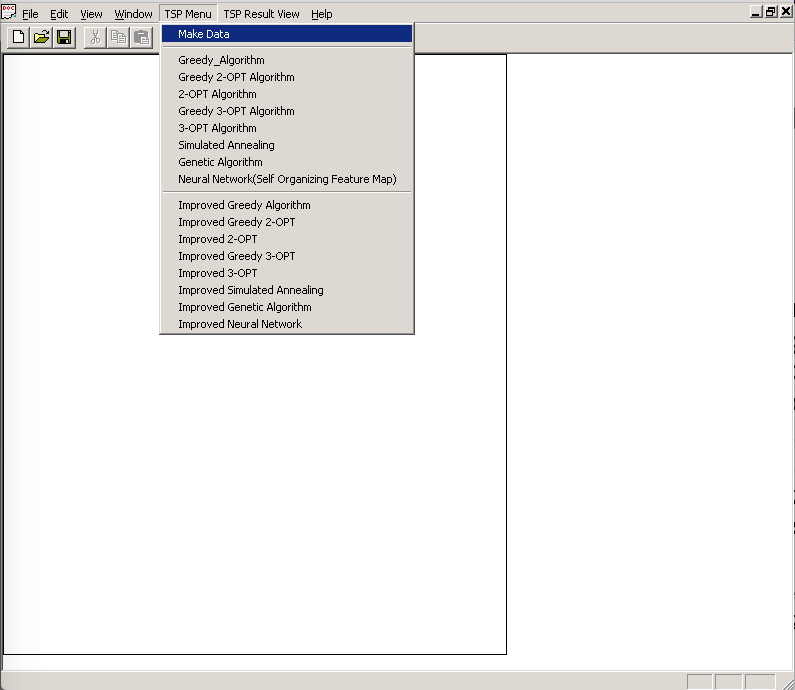
\includegraphics[width=8cm]{TSPProgram.png}
\captionof{figure}{Traveling Salesman Problem Software from MFC library}
\end{center}

\newpage
\section{Experiment}
To do an experiment, TSP simulation program\cite{TSPProgram} was used and compared the length of the route depending on the number of the cities for each heuristic algorithms that was mentioned. For the number of cities, I used 48, 220 and 452. These numbers represent the real number of cities for population between 250000 to 499999, 100000-249999 and 50000 to 99999 each and data are from \enquote{Statista}.\cite{statista} 
\begin{itemize}
\item Greedy Algorithm
		\begin{center}
			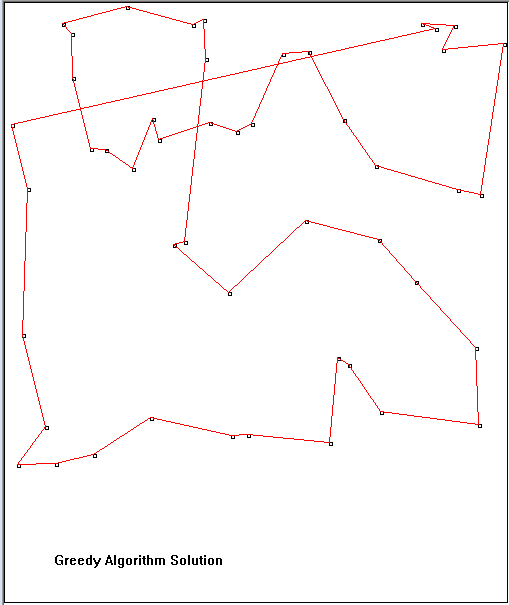
\includegraphics[width=5cm]{Greedy48.png}
            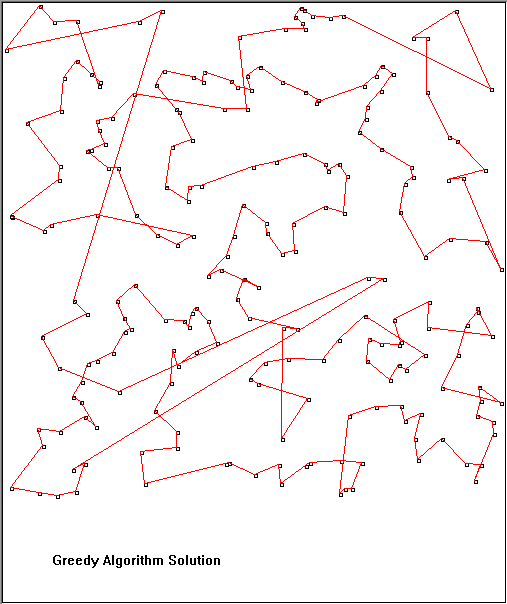
\includegraphics[width=5cm]{Greedy220.PNG}
            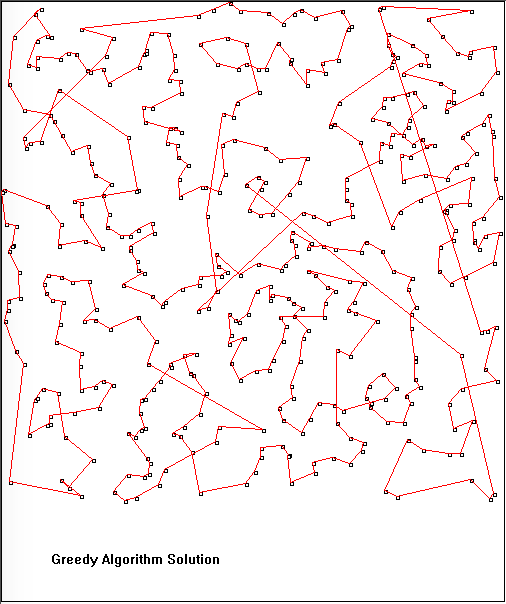
\includegraphics[width=5cm]{Greedy452.png}
            \captionof{figure}{Greedy Algorithm Simulation for city size of 48, 220, 452}
		\end{center}

For the Greedy Algorithm on TSP, the length of the route was 3213.31, 6996.35 and 12558.14 for the city size of 48, 220 and 452 each. The runtime for the algorithm to be run in each size were shown as $0$, meaning it took really short time that is close to $0$ $sec$.

\item Neural Network
		\begin{center}
			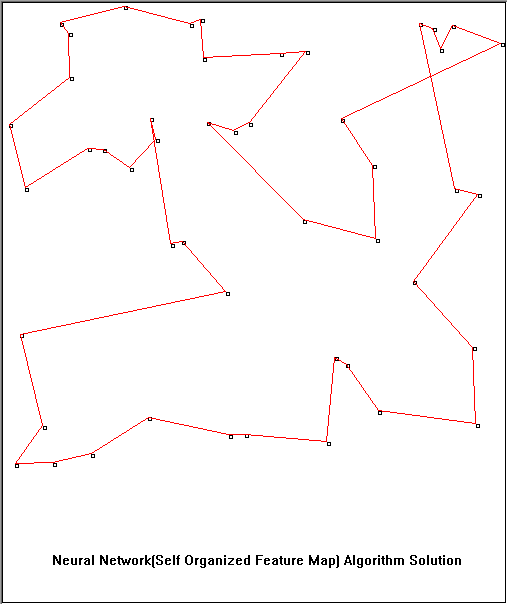
\includegraphics[width=5cm]{Neural48.PNG}
            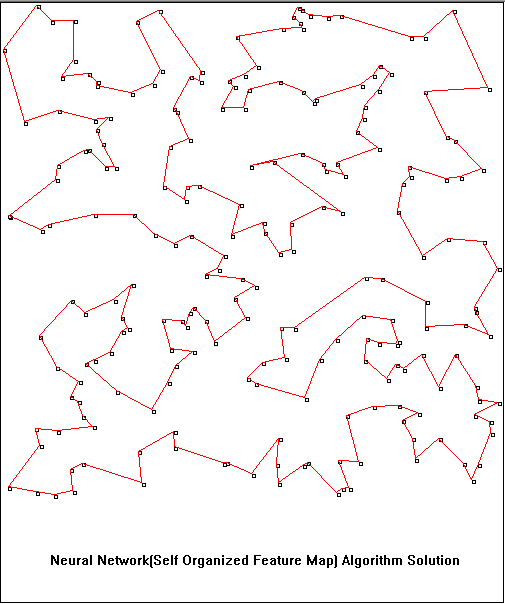
\includegraphics[width=5cm]{Neural220.PNG}
            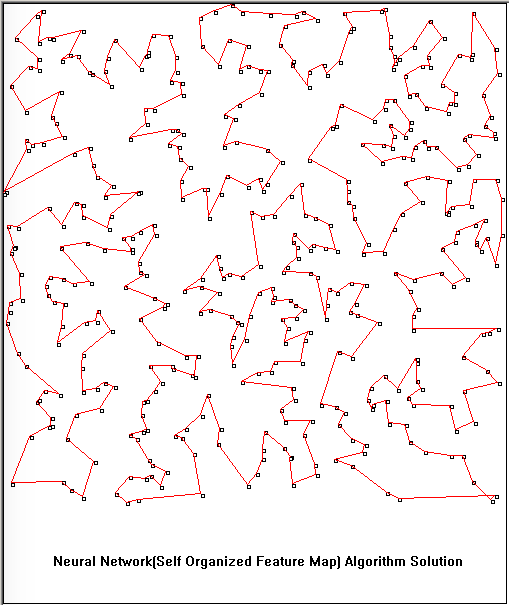
\includegraphics[width=5cm]{Neural452.png}
            \captionof{figure}{Neural Network Simulation for city size of 48, 220, 452}
		\end{center}

For the Neural Network on TSP, the length of the route was 3025.14, 5648.83 and 8268.67 for the city size of 48, 220 and 452 each. The runtime for the algorithm to be run in each size were 1 $sec$, 6 $sec$ and 44 $sec$ each. 

\item Simulated Annealing
		\begin{center}
			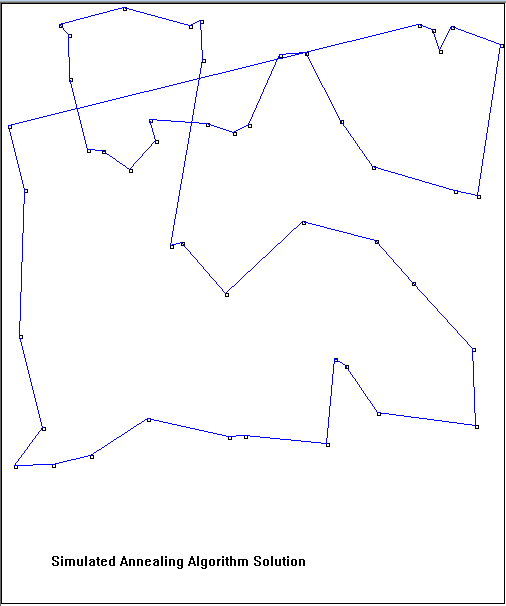
\includegraphics[width=5cm]{Simulated48.PNG}
            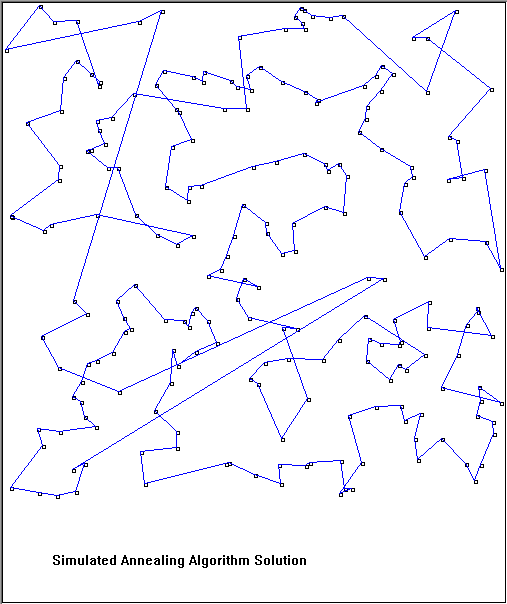
\includegraphics[width=5cm]{Simulated220.PNG}
            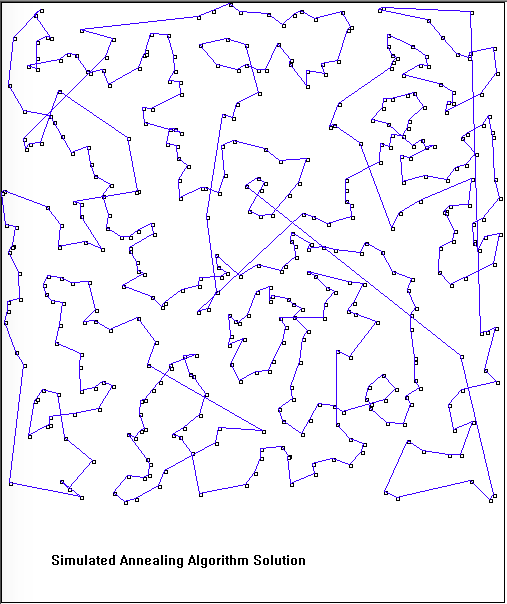
\includegraphics[width=5cm]{Simulated452.png}
            \captionof{figure}{Simulated Annealing Simulation for city size of 48, 220, 452}
		\end{center}
        
For the Simulated Annealing on TSP, the length of the route was 3168.28, 6927.64 and 9729.60 for the city size of 48, 220 and 452 each. The runtime for the algorithm to be run in each size were 0 $sec$ for sample size of 48, 220 and 3 $sec$ for size 452. 

\item Improved Greedy Algorithm
		\begin{center}
			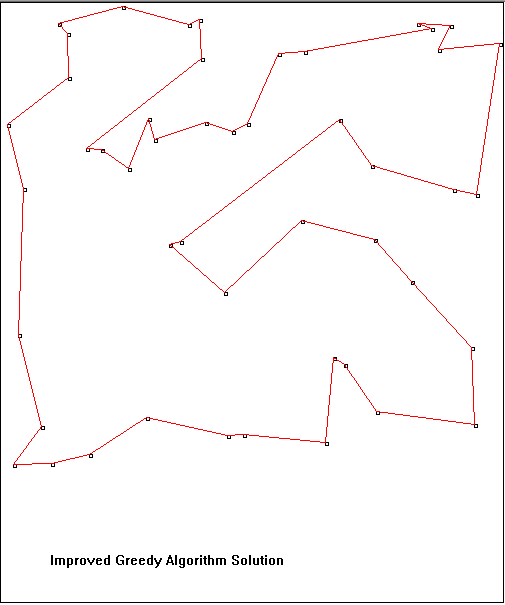
\includegraphics[width=5cm]{ImprovedGreedy48.PNG}
            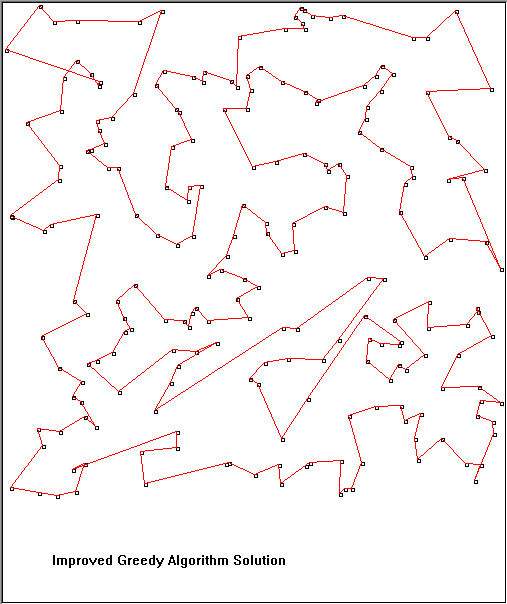
\includegraphics[width=5cm]{ImprovedGreedy220.PNG}
            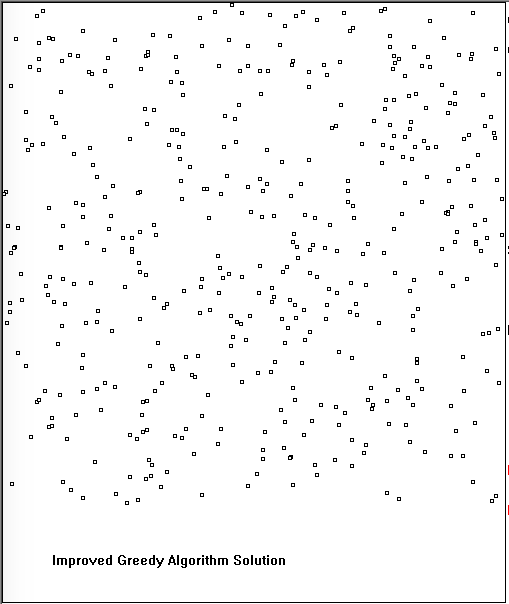
\includegraphics[width=5cm]{ImprovedGreedy452.png}
            \captionof{figure}{Improved Greedy Algorithm Simulation for city size of 48, 220, 452}
		\end{center}

For the improved version of Greedy Algorithm on TSP, the length of the route was 2997.26 and 6274.73 for the city size of 48 and 220 each. In case of the city size of 452, the improved greedy algorithm could not calculate the length of the route by the program I used. 

\item Improved Neural Network
		\begin{center}
			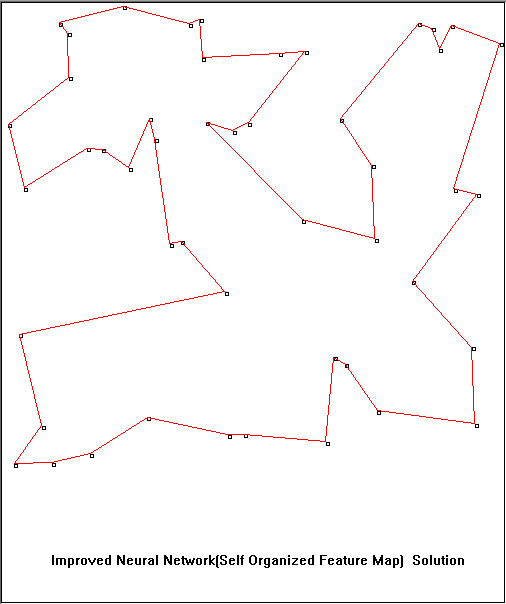
\includegraphics[width=5cm]{ImprovedNeural48.PNG}
            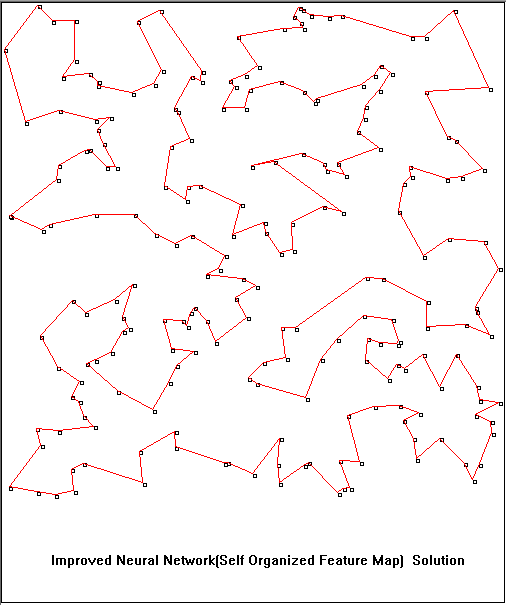
\includegraphics[width=5cm]{ImprovedNeural220.PNG}
            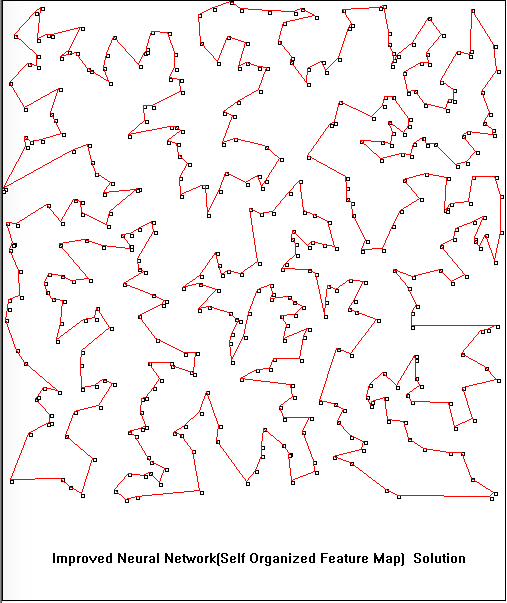
\includegraphics[width=5cm]{ImprovedNeural452.png}
            \captionof{figure}{Improved Neural Network Simulation for city size of 48, 220, 452}
		\end{center}
        
For the improved version of Neural Network on TSP, the length of the route was 2949.29, 5648.83 and 8265.25 for the city size of 48, 220 and 452 each.         
        
\item Improved Simulated Annealing
		\begin{center}
			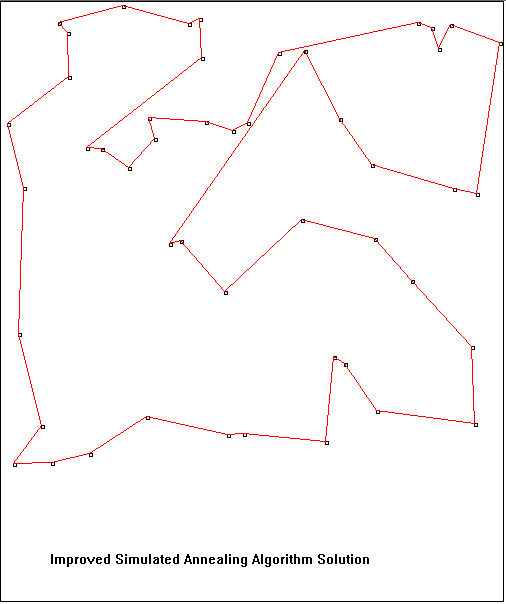
\includegraphics[width=5cm]{ImprovedSimulated48.PNG}
            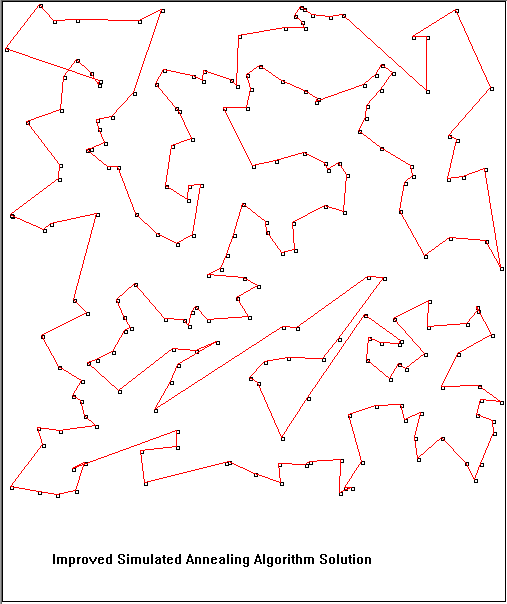
\includegraphics[width=5cm]{ImprovedSimulated220.PNG}
            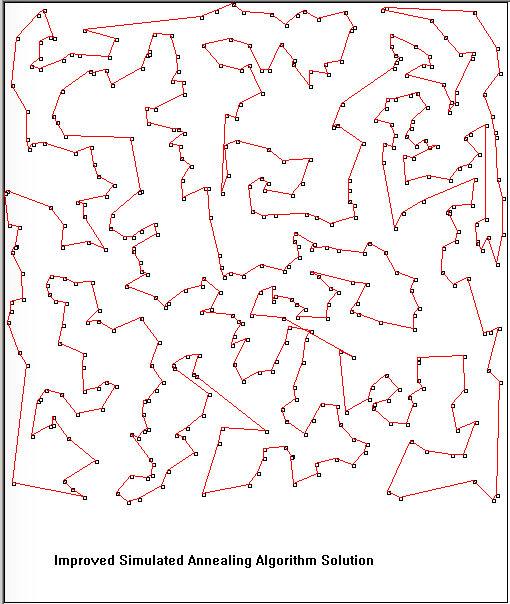
\includegraphics[width=5cm]{ImprovedSimulated452.png}
            \captionof{figure}{Improved Simulated Annealing Simulation for city size of 48, 220, 452}
		\end{center}        

For the improved version of Simulated Annealing on TSP, the length of the route was 3058.74, 6302.49 and 8947.13 for the city size of 48, 220 and 452 each.

\end{itemize}

\section{Analysis}

By doing experiment with 3 heuristic algorithms, which are Greedy algorithm, Neural Network and Simulated Annealing and as well as improved version of each algorithms, we could compare the length of the route and runtime on TSP. The tables and graph shown below describe the comparison of each algorithms. \par

According to the $Table$ $1$, we can observe that the Neural Network has the least amount of distance for all 3 of the city sizes. The $Table$ $2$ shows the improved version of each algorithms. Compared to the regular heuristic algorithms, each improved version for 3 algorithms yield shorter length of the route. And we can observe that improved version of Neural Network still has the shortest length. And we can observe that the difference between regular algorithm and improved algorithm on route length, Neural Network has the least difference. The reason that the improved algorithm comes out with the shorter length of route is because it removes the crossings that each algorithms make.
\begin{displaymath}
    \begin{array} {|p{5cm}||p{3cm}|p{3cm}|p{3cm}|}
  	  \hline
      \multirow{2}{*}{Algorithms} & \multicolumn{3}{c|}{City Size} \\
      \cline{2-4}
      & 48 & 220 & 452 \\
      \hline
      Greedy Algorithm & 3213.31 & 6996.35 & 9741.05 \\
      \hline
      Neural Network & 3025.14 & 5648.83 & 8268.87 \\
      \hline
      Simulated Annealing & 3168.28 & 6927.64 & 9729.60 \\
      \hline
    \end{array}
  \end{displaymath}
	\captionof{table}{Length of the Route on each Algorithms}

    \begin{displaymath}
    \begin{array} {|p{5cm}||p{3cm}|p{3cm}|p{3cm}|}
  	  \hline
      \multirow{2}{*}{Algorithms} & \multicolumn{3}{c|}{City Size} \\
      \cline{2-4}
      & 48 & 220 & 452 \\
      \hline
      Improved Greedy Algorithm & 2997.26 & 6274.73 & - \\
      \hline
      Improved Neural Network & 2949.29 & 5648.83 & 8265.25 \\
      \hline
      Improved Simulated Annealing & 3058.74 & 6302.49 & 8947.13 \\
      \hline
    \end{array}
  \end{displaymath}
	\captionof{table}{Length of the Route on each Algorithms}

	\begin{center}
            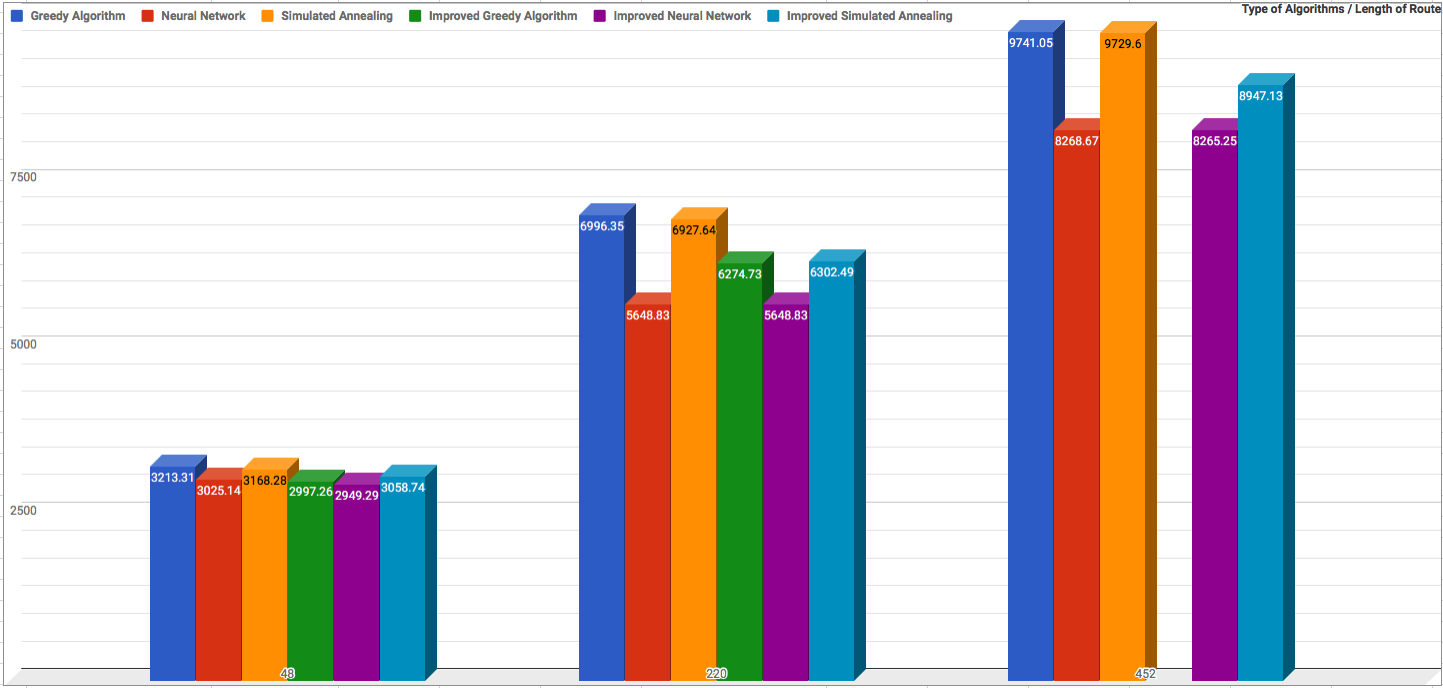
\includegraphics[width=12cm]{RouteLength.png}
            \captionof{figure}{Comparison of Length of Route}
		\end{center}  

As can be observed from the figure, the greedy algorithm has a long line of crossing from left to right. The improved version of greedy algorithm, efficiently removed the crossing and made the total length of the route to be shorter.

\begin{center}
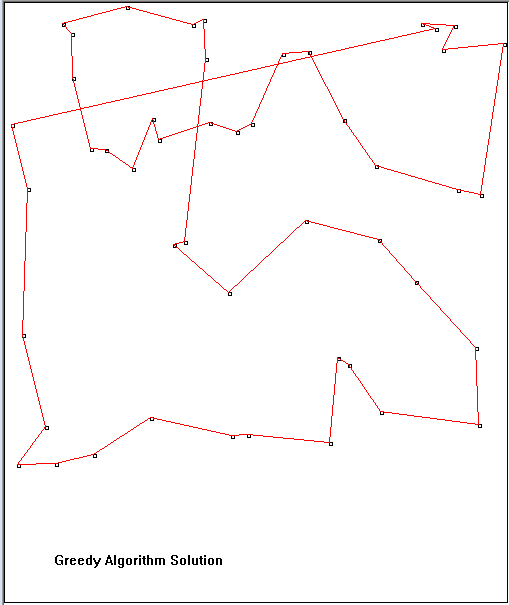
\includegraphics[width=5cm]{Greedy48.png}
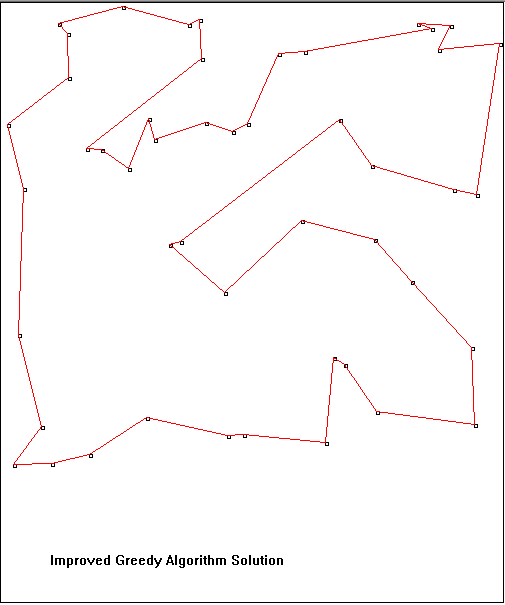
\includegraphics[width=5cm]{ImprovedGreedy48.PNG}
\captionof{figure}{Comparison of Greedy and Improved Greedy Algorithm}
\end{center}

In terms of runtime, Greedy Algorithm came out with the result right away, which shows as 0 sec. Neural Network, it took the longest time among 3 algorithms that was experimented. In case of Simulated Annealing, when the city size was 48 and 220, it took really short time that is close to 0 sec and when the city size was 452 which was quite big, it took 3 sec. 
\par

During the experiment, the result of improved version of Greedy Algorithm on city size of 452 was not shown. In the program, \enquote{Resolving cross 452/452} message comes out and it took longer than 1 hour and still cannot find the solution. Compared to runtime of any other heuristic algorithm, improved greedy algorithm took too much that it was meaningless to wait couple hours for the result.

\begin{displaymath}
    \begin{array} {|p{5cm}||p{3cm}|p{3cm}|p{3cm}|}
  	  \hline
      \multirow{2}{*}{Algorithms} & \multicolumn{3}{c|}{City Size} \\
      \cline{2-4}
      & 48 & 220 & 452 \\
      \hline
      Greedy Algorithm & 0 & 0 & 0 \\
      \hline
      Neural Network & 1 & 6 & 44 \\
      \hline
      Simulated Annealing & 0 & 0 & 3 \\
      \hline
    \end{array}
  \end{displaymath}
    \captionof{table}{Runtime of each Algorithm}
\newpage
\section{Conclusion}
In order to solve Traveling Salesman Problem(TSP), there were 3 heuristic algorithms used. Greedy Algorithm, Neural Network and Simulated Annealing. Also, to get better result, there were improved version of each 3 algorithms are used as well. In terms of finding the shortest length of route, Neural Network was the most suitable heuristic algorithm for TSP since it came out with the shortest length of the route whatever the city size was. Also for the improved version of each heuristic algorithm, Neural Network had the shortest route length for all city size. In terms of the runtime for each algorithm however, Neural Network took much longer than 2 other algorithms that was experimented and Greedy algorithm was the most efficient. \newline
When simulating the improved version of greedy algorithm, when city size was big, which was 452 in this case, the program could not find the solution for the TSP. Unofficially, the experiment for the improved greedy algorithm for city size of 300 was done and it seemed like it is showing an error on finding the solution.
\begin{center}
            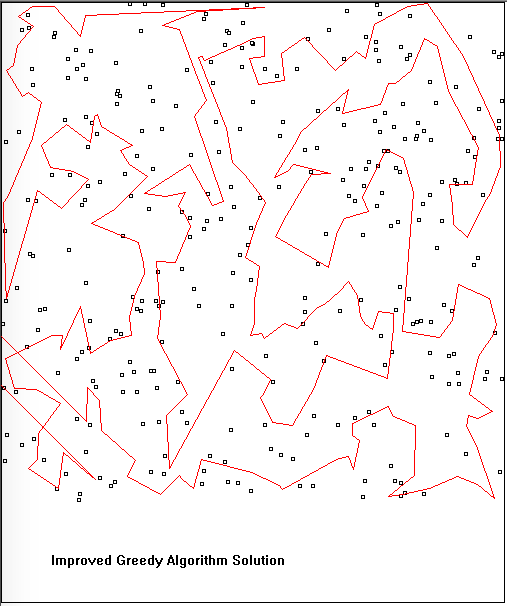
\includegraphics[width=5cm]{ImprovedGreedy300.png}
            \captionof{figure}{Improved version of Greedy Algorithm on City Size of 300}
		\end{center}  
For later, there needs an experiment to figure out the reason that the improved version of Greedy Algorithm cannot find the solution. Also, in this paper, the experiment was done for only 3 heuristic algorithms. But there exists more heuristic algorithms that can be useful in TSP such as 2-opt, 3-opt and Genetic algorithm.\cite{Genetic} If there are more algorithms to be compared, we can come out with more accurate result so that in the future, more examples will follow as well as the revision of current algorithm used in this paper. 
\newpage
\bibliographystyle{plain}
\bibliography{references}
\end{document}

